% Generated by book/tools/notebook_to_tex.py. Do not edit by hand.

\chapter[한국어 Diffusion LM]{한국어 Diffusion LM: 80/10/10 마스킹}

\label{ch:34}

\markboth{한국어 Diffusion LM}{한국어 Diffusion LM}

\chaptermeta{34_ko_diffusion/34_ko_diffusion.ipynb}{https://colab.research.google.com/github/yoon-gu/neuqes-101/blob/master/34_ko_diffusion/34_ko_diffusion.ipynb}{한국어 TinyStories에서 diffusion LM을 학습하며 naive 마스킹 붕괴와 BERT식 80/10/10 마스킹을 비교}



\index{1Korean Diffusion LM@Korean Diffusion LM}

\index{1BERT 80 10 10 masking@BERT 80/10/10 masking}

\index{1ByteLevel BPE@ByteLevel BPE}

\index{1TinyStories Korean@TinyStories-Korean}

\index{1unigram collapse@unigram collapse}

\index{1plain CE@plain CE}

\index{1fixed t accuracy@fixed-t accuracy}

\index{0한국어 diffusion@한국어 diffusion}

\index{0한국어 BBPE@한국어 BBPE}

\index{0BERT식 마스킹@BERT식 마스킹}

\index{0유니그램 붕괴@유니그램 붕괴}

\index{0복원 정확도@복원 정확도}



\section{작은 diffusion LM으로 한국어 동화 만들기 --- 80/10/10 마스킹}

이 장에서는 직전 영어 장와 똑같은 4.29M짜리 작은 mask-diffusion 언어 모델로 한국어 동화를 생성합니다. 전부 \texttt{{[}MASK{]}}로 채운 빈 캔버스에서 출발해도, 학습을 마친 모델은 이런 이야기를 끝까지 이어 씁니다.

\begin{quote}
옛날 옛적에 팀이라는 작은 소년이 있었어요. 팀은 장난감 가지고 노는 것을 매우 좋아했지요\ldots{}
\end{quote}

\begin{quote}
공원에 도착해서 맥스는 맥스라는 큰 공을 봤어요. “와, 정말 멋진 공이야! 우리 공으로 같이 놀자!”\ldots{}
\end{quote}

인물과 대화, 배경과 서사가 모두 들어 있습니다. 고정 마스킹 비율 \(t=0.15\)에서 빈칸 복원 top-1 정확도는 0.652까지 올라가고(영어 33장은 0.717), \inlinecode{train\_loss}는 4.13까지 내려갑니다.

이 결과를 만든 핵심은 \textbf{BERT가 원래 쓰던 80/10/10 마스킹} 한 가지입니다. 마스킹 대상 자리를 전부 \texttt{{[}MASK{]}}로 바꾸지 않고, 80\%만 \texttt{{[}MASK{]}}로 두고 10\%는 랜덤 토큰, 10\%는 원본 그대로 둡니다. 영어 33장과 모델·데이터 규모는 같고, 한국어에서 결정적으로 달라지는 건 이 마스킹뿐입니다. 왜 이 한 가지가 한국어에서 그토록 결정적인지는, 실습으로 동작하는 결과를 먼저 본 뒤 \textbf{해부} 절에서 순진한 100\% \texttt{{[}MASK{]}} 방식과 직접 대조하며 규명합니다.



\section{추적표 (Phase 5 --- diffusion 라인)}

\begin{booktable}{34장 추적표 (Phase 5 - diffusion 라인) 표}{tab:ch34-01}
\begin{adjustbox}{max width=\textwidth}
\begin{tabular}{@{}lllll@{}}
\toprule
장 & 언어 & 토크나이저 & 마스킹 방식 & 결과 \\
\midrule

33장 (성공) & 영어 (TinyStories) & ByteLevel BPE, vocab 2048 & 100\% \texttt{{[}MASK{]}} & train\_loss 낮고 생성 coherent, top-1 acc 0.717 \\
\textbf{34장 (해결)} & \textbf{한국어 (TinyStories-Korean)} & \textbf{ByteLevel BPE, vocab 4000} & \textbf{80/10/10 (\texttt{{[}MASK{]}} / 랜덤 / 원본)} & \textbf{순진한 이식은 train\_loss 7.06 · acc 0.081로 붕괴 \(\to\) 80/10/10으로 train\_loss 4.13 · acc 0.652 회복, 생성 coherent} \\
\bottomrule
\end{tabular}
\end{adjustbox}
\end{booktable}

33장과 34장의 모델 본체(\inlinecode{BertForMaskedLM}, hidden 256/4L/4H, \textasciitilde4.29M)와 샘플러(carry-over semi-AR, block 32 + 반복억제)는 같습니다. 바뀐 것은 학습 언어와, 그 변화가 드러낸 마스킹 방식 하나입니다. 영어에서 100\% \texttt{{[}MASK{]}}로도 버티던 레시피가 한국어에서 무너지고, 마스킹 대상의 일부를 랜덤 토큰과 원본으로 섞는 80/10/10을 적용하자 손실의 벽 7.0을 완전히 돌파합니다.



\section{변경점: 33장 대비}

\begin{booktable}{34장 변경점 요약}{tab:ch34-02}
\begin{adjustbox}{max width=\textwidth}
\begin{tabular}{@{}llll@{}}
\toprule
항목 & 이전 (33장) & 이번 (34장) & 왜 바꾸나 \\
\midrule

언어 & 영어 & 한국어 & 33장의 영어 성공 레시피가 한국어에서도 통하는지 확인하려는 것이 출발점입니다. 결과적으로 이 변화가 마스킹 방식의 숨은 결함을 끌어냈습니다. \\
데이터 & TinyStories & TinyStories-Korean (\inlinecode{g0ster/TinyStories-Korean}, 50,000 stories \(\to\) 75,941 chunks, 약 9.7M 토큰) & \ref{ch:26}장 한국어 AR과 같은 코퍼스를 써서 “같은 데이터로 AR은 되는데 diffusion은 왜 안 되나”를 일관되게 대조하기 위해서입니다. \\
vocab & 2048 & 4000 & 한국어는 조사·어미가 붙는 교착어라 영어보다 토큰 다양성이 커서 vocab을 약간 키웁니다. \ref{ch:26}장 한국어 AR도 4000을 썼습니다. \\
마스킹 & 100\% \texttt{{[}MASK{]}} & 80/10/10 (80\% \texttt{{[}MASK{]}}, 10\% 랜덤 토큰, 10\% 원본 유지) & 한국어는 조사·어미의 유니그램 예측성이 높아, “{[}MASK{]}면 고빈도 토큰 찍기” 지름길의 유혹이 영어보다 훨씬 강합니다. 마스킹 대상에 랜덤·원본을 섞어 그 지름길을 막아야 모델이 문맥을 실제로 학습합니다. \\
\bottomrule
\end{tabular}
\end{adjustbox}
\end{booktable}

핵심 메시지는 이렇습니다. 우리는 언어 하나만 바꾼 줄 알았는데, 그 변화가 마스킹 방식의 결함을 드러냈습니다. 영어 TinyStories는 어휘와 구문이 단순하고 반복적이라 100\% \texttt{{[}MASK{]}}만으로도 모델이 문맥을 배울 여지가 있었습니다. 한국어는 같은 자리를 조사·어미의 빈도만으로 그럴듯하게 채울 수 있어, 100\% \texttt{{[}MASK{]}}는 모델에게 “주변을 안 봐도 되는” 지름길을 열어 줍니다. 그래서 변경점은 표면상 “언어” 하나지만, 실질적으로는 그 언어가 끌어낸 “마스킹 방식”까지 두 칸이 함께 움직인 장입니다.



\section{마스킹 노트 --- 80/10/10이 한국어 diffusion의 정답}

이번 장의 학습 코드는 마스킹 대상으로 뽑힌 자리를 전부 \texttt{{[}MASK{]}}로 바꾸지 않습니다. BERT가 원래 쓰던 비율 그대로 셋으로 나눕니다.

\begin{itemize}
\tightlist
\item
  \textbf{80\% \(\to\) \texttt{{[}MASK{]}}} --- 일반적인 빈칸 복원
\item
  \textbf{10\% \(\to\) 랜덤 토큰} --- 엉뚱한 토큰으로 바꿔놓고 정답을 맞히게 함
\item
  \textbf{10\% \(\to\) 원본 그대로 유지} --- 입력은 멀쩡한데 그 자리에도 손실이 걸림
\end{itemize}

핵심은 두 소수파가 하는 일입니다. \textbf{10\% 원본 유지}는 “정답을 맞혀야 하는 자리가 꼭 \texttt{{[}MASK{]}}인 것은 아니다”라고 알려줍니다. 모델은 \texttt{{[}MASK{]}} 표식에만 기대 답을 고를 수 없고, 멀쩡해 보이는 토큰도 문맥과 맞는지 매번 검증해야 합니다. \textbf{10\% 랜덤 토큰}은 “눈에 보이는 입력이 틀렸을 수 있으니 교정하라”고 강제합니다. 입력을 그대로 믿는 대신 문맥과 대조하는 습관이 생깁니다. 두 장치가 합쳐지면 모델은 표식이 아니라 문맥을 읽게 됩니다.

\subsection{수치 예시 --- 128토큰 시퀀스에서 어떻게 쪼개지는가}

마스킹 비율 \(t\)를 뽑으면 시퀀스 길이 \(L=128\)에 대해 약 \(tL\)개 자리가 마스킹 대상이 되고, 그 안에서 다시 80/10/10으로 나뉩니다.

\begin{booktable}{34장 손실 수치 예시}{tab:ch34-03}
\begin{adjustbox}{max width=\textwidth}
\begin{tabular}{@{}ccccc@{}}
\toprule
마스킹 비율 \(t\) & 마스킹 대상 (\(\approx tL\)) & \texttt{{[}MASK{]}} (80\%) & 랜덤 (10\%) & 원본 유지 (10\%) \\
\midrule

0.15 & 20 & 16 & 2 & 2 \\
0.30 & 38 & 31 & 4 & 4 \\
0.50 & 64 & 51 & 6 & 6 \\
\bottomrule
\end{tabular}
\end{adjustbox}
\end{booktable}

(마스킹 대상 수와 80/10/10 분해는 반올림 때문에 합이 ±1 어긋날 수 있습니다. \(t=0.15\) 행만 16+2+2=20으로 정확히 떨어집니다.)

표를 보면 \(t=0.15\)에서 정답을 맞혀야 하는 20개 자리 중 4개(랜덤 2 + 원본 2)는 \texttt{{[}MASK{]}} 표식이 아예 없습니다. 이 4개가 모델에게 “표식이 아니라 문맥을 보라”고 끊임없이 압박하는 장치입니다. 가변 마스킹 \(t \sim U(0.05, 1)\)은 직전 장 그대로 유지합니다.

손실은 이 마스킹 대상 자리들의 평균 교차 엔트로피로 계산합니다. 직전 장에서 쓰던 시간 가중 \(1/t\)는 기댓값 상 마스크 토큰당 평균 CE와 상수배로 같으므로, 여기서는 표준 MLM과 눈높이를 맞추기 위해 가중 없는 plain CE(\inlinecode{BertForMaskedLM} 기본)를 그대로 씁니다.

\subsection{\texorpdfstring{순진한 100\% \texttt{{[}MASK{]}}는 지름길을 연다}{순진한 100\% {[}MASK{]}는 지름길을 연다}}

같은 모델·데이터에서 마스킹 대상을 전부 \texttt{{[}MASK{]}}로만 바꾸면, 모델은 두 가지를 알아챕니다. 정답을 맞혀야 하는 자리는 \textbf{항상} \texttt{{[}MASK{]}} 자리이고, \texttt{{[}MASK{]}} 자체엔 의미가 없으니 주변만 보면 된다는 것입니다. 한국어는 조사(“-가”, “-를”, “-에”)와 어미(“-요”, “-어요”, “-습니다”)의 빈도가 압도적으로 높아, 문맥을 거의 안 보고 고빈도 토큰만 찍어도 손실이 빠르게 떨어집니다. 그래서 모델은 “\texttt{{[}MASK{]}}면 흔한 토큰 찍기”라는 유니그램 지름길에 멈춥니다. 균등하게 찍을 때의 손실이 \(\ln 4000 \approx 8.29\)인데, 이 지름길은 빈도 정보만큼만 내려간 자리에서 정체합니다.

80/10/10의 10\% 원본 유지(문맥 검증 강제)와 10\% 랜덤(교정 강제)이 바로 이 지름길을 막습니다. 그래서 한국어 diffusion에서는 이 마스킹이 선택이 아니라 정답입니다.

이 한 가지 수정으로 \inlinecode{train\_loss}가 4.13까지 내려가고 고정-\(t\)(0.15) top-1 정확도가 0.081에서 0.652로 뜁니다. 곧 실습에서 직접 확인합니다.



\section{토크나이저 노트}

이 장은 ByteLevel BPE 토크나이저를 직접 학습해서 씁니다. 어휘 수는 4000으로, 영어 직전 장의 2048보다 키웠습니다. 한국어는 조사와 어미가 어간에 붙는 교착어라 같은 어근도 표면형이 다양하게 늘어나기 때문에, 어휘가 너무 작으면 토큰이 잘게 부서져 한 문장의 토큰 수가 불필요하게 길어집니다. 한국어 자기회귀 모델을 다룬 장에서도 같은 4000을 썼습니다.

ByteLevel 방식은 텍스트를 일단 바이트 단위로 본 뒤 그 위에서 BPE 병합을 학습합니다. 학습 시 \inlinecode{initial\_alphabet}으로 256개 바이트를 전부 포함시켜 두기 때문에, 어떤 한글 음절이나 처음 보는 문자가 들어와도 최소한 바이트 단위로는 항상 표현할 수 있습니다. 덕분에 \texttt{{[}UNK{]}}로 빠지는 경우가 사실상 사라집니다. 여기에 마스크 학습과 패딩에 필요한 특수 토큰 \texttt{{[}PAD{]}}, \texttt{{[}UNK{]}}, \texttt{{[}MASK{]}}를 더했습니다. \texttt{{[}MASK{]}}는 이 장의 80/10/10 마스킹에서 핵심 역할을 합니다.

예를 들어 “옛날 옛날에 작은 토끼가 숲으로 갔어요”라는 문장을 토큰화하면, “옛날”, “작은”처럼 자주 등장하는 덩어리는 하나의 토큰으로 묶이고, 드문 글자나 조사 경계는 더 작은 서브워드 또는 바이트 조각으로 쪼개집니다. 같은 어근이라도 “갔어요”, “갔다”처럼 어미가 달라지면 뒤쪽 토큰이 갈라지는데, 어휘를 4000까지 확보한 덕에 흔한 어미 패턴은 통째로 한 토큰으로 유지되어 시퀀스가 지나치게 길어지지 않습니다.



\section{실습 --- 직접 학습하고 생성해 보기}

80/10/10 콜레이터로 작은 모델을 학습시켜 한국어 동화를 생성해 봅니다. (80/10/10이 무엇인지는 위 마스킹 노트에서 봤고, 순진한 100\% \texttt{{[}MASK{]}}가 왜 무너지는지는 뒤 해부에서 다룹니다.) T4에서 30000 step, 약 20분.



\Needspace{5\baselineskip}
\begin{lstlisting}
%pip install -q -U transformers tokenizers datasets accelerate
\end{lstlisting}

\begin{codeRead}
\textbf{1행}의 \inlinecode{\%pip install -q -U transf...}에서는 앞 단계에서 만든 값을 바탕으로 다음 계산을 수행합니다.
\end{codeRead}



\Needspace{9\baselineskip}
\begin{lstlisting}
import math, time, torch
import torch.nn.functional as F
from datasets import load_dataset, Dataset
SEED=42; torch.manual_seed(SEED)
device = "cuda" if torch.cuda.is_available() else ("mps" if torch.backends.mps.is_available() else "cpu")
USE_FP16 = torch.cuda.is_available()
print("device", device, "| fp16", USE_FP16)
\end{lstlisting}

\begin{codeRead}
\inlinecode{PyTorch, datasets} 같은 주요 패키지를 불러옵니다. \textbf{4행}의 \inlinecode{SEED = ...}에서는 이후 분석에서 사용할 값을 준비합니다. \textbf{5행}의 \inlinecode{device = ...}에서는 이후 분석에서 사용할 값을 준비합니다. \textbf{6행}의 \inlinecode{USE\_FP16 = ...}에서는 이후 분석에서 사용할 값을 준비합니다.
\end{codeRead}

\noindent\textbf{출력.}
\begin{bookoutputbox}
device cuda | fp16 True
\end{bookoutputbox}
\par\vspace{0.9em}



\subsection{한국어 TinyStories 복원 (\ref{ch:26}장과 동일)}



\Needspace{11\baselineskip}
\begin{lstlisting}
EOT="<|endoftext|>"; N_TRAIN,N_VAL,MAXL=50_000,500,1_500_000
def rebuild(split,n,maxl):
    stories,buf=[],[]
    for i,ex in enumerate(load_dataset("g0ster/TinyStories-Korean",split=split,streaming=True)):
        if i>=maxl or len(stories)>=n: break
        line=(ex["text"] or "").strip()
        if line==EOT:
            s=" ".join(buf).strip()
            if s: stories.append(s)
            buf=[]
        elif line: buf.append(line)
    if buf and len(stories)<n:
        s=" ".join(buf).strip()
\end{lstlisting}

\noindent\emph{앞 블록은 데이터를 불러오고 학습에 맞는 형태로 정리하는 단계입니다. 이어지는 블록에서는 앞에서 만든 중간 값을 다음 계산으로 넘기는 단계로 넘어갑니다.}

\Needspace{8\baselineskip}
\begin{lstlisting}[firstnumber=14]
        if s: stories.append(s)
    return stories[:n]
raw_train=Dataset.from_dict({"text":rebuild("train",N_TRAIN,MAXL)})
raw_val=Dataset.from_dict({"text":rebuild("validation",N_VAL,50_000)})
print("stories", len(raw_train), len(raw_val))
print(raw_train[0]["text"][:120])
\end{lstlisting}

\noindent\textbf{출력.}
\begin{bookoutputbox}
If the error persists, please let us know by opening an issue on GitHub (ht...
stories 50000 500
한때 벤이라는 이름의 어린 소년이 있었어요. 벤은 주변 세계를 탐험하는 것을...
\end{bookoutputbox}
\par\vspace{0.9em}



\subsection{BPE 4000 + initial\_alphabet + {[}MASK{]}}



\Needspace{11\baselineskip}
\begin{lstlisting}
from tokenizers import Tokenizer, models, trainers, pre_tokenizers, decoders
from transformers import PreTrainedTokenizerFast
VOCAB=4000
def corpus_iter(bs=1000):
    for i in range(0,len(raw_train),bs): yield raw_train[i:i+bs]["text"]
_tk=Tokenizer(models.BPE(unk_token="[UNK]"))
_tk.pre_tokenizer=pre_tokenizers.ByteLevel(add_prefix_space=False)
_tk.decoder=decoders.ByteLevel()
_tk.train_from_iterator(corpus_iter(), trainer=trainers.BpeTrainer(
    vocab_size=VOCAB, special_tokens=["[PAD]","[UNK]","[MASK]"],
    initial_alphabet=pre_tokenizers.ByteLevel.alphabet()))
tokenizer=PreTrainedTokenizerFast(
    tokenizer_object=_tk,
    pad_token="[PAD]",
    unk_token="[UNK]",
    mask_token="[MASK]",
\end{lstlisting}

\noindent\emph{앞 블록은 필요한 라이브러리와 기본 설정을 준비하는 단계입니다. 이어지는 블록에서는 텍스트를 모델 입력 텐서로 바꾸는 단계로 넘어갑니다.}

\Needspace{6\baselineskip}
\begin{lstlisting}[firstnumber=17]
)
print(
    "vocab", tokenizer.vocab_size, "mask_id", tokenizer.mask_token_id
)
\end{lstlisting}

\noindent\textbf{출력.}
\begin{bookoutputbox}
vocab 4000 mask_id 2
\end{bookoutputbox}
\par\vspace{0.9em}



\subsection{토큰화 + group}



\Needspace{11\baselineskip}
\begin{lstlisting}
BLOCK=128
tt=raw_train.map(
    lambda b: tokenizer(b["text"],add_special_tokens=False),
    batched=True,
    remove_columns=raw_train.column_names,
)
tv=raw_val.map(
    lambda b: tokenizer(b["text"],add_special_tokens=False),
    batched=True,
    remove_columns=raw_val.column_names,
)
\end{lstlisting}

\noindent\emph{앞 블록은 텍스트를 모델 입력 텐서로 바꾸는 단계입니다. 이어지는 블록에서는 앞에서 만든 중간 값을 다음 계산으로 넘기는 단계로 넘어갑니다.}

\Needspace{11\baselineskip}
\begin{lstlisting}[firstnumber=12]
def group(b):
    cat=sum(b["input_ids"],[]); n=(len(cat)//BLOCK)*BLOCK
    return {"input_ids":[cat[i:i+BLOCK] for i in range(0,n,BLOCK)]}
lm_train=tt.map(
    group,
    batched=True,
    remove_columns=tt.column_names,
)
lm_val=tv.map(
    group,
    batched=True,
    remove_columns=tv.column_names,
)
print("chunks", len(lm_train), len(lm_val))
\end{lstlisting}

\noindent\textbf{출력.}
\begin{bookoutputbox}
chunks 75941 746
\end{bookoutputbox}
\par\vspace{0.9em}



\subsection{수정 --- diffusion 콜레이터에 80/10/10 (순진한 100\% {[}MASK{]} 대신)}

가변 마스킹률 t는 유지(생성용)하되, 선택된 자리에 80\% {[}MASK{]} / 10\% 랜덤 / 10\% 원본유지. 이게 모델이 {[}MASK{]}\(\to\)유니그램 지름길로 새는 걸 막는다.



\Needspace{11\baselineskip}
\begin{lstlisting}
N_SPECIAL=3
class DiffMLMCollator:
    def __init__(self, tok, eps=0.05, tmax=1.0, seed=SEED):
        self.mask_id=tok.mask_token_id; self.vocab=tok.vocab_size
        self.eps=eps; self.tmax=tmax; self.gen=torch.Generator().manual_seed(seed)
    def __call__(self, ex):
        ids=torch.tensor(
            [e["input_ids"] for e in ex],
            dtype=torch.long,
        )
        B,L=ids.shape
        t=torch.rand(B,generator=self.gen)*(self.tmax-self.eps)+self.eps
        sel=torch.rand(
            B,
            L,
            generator=self.gen)<t.unsqueeze(1,
\end{lstlisting}

\noindent\emph{앞뒤 블록은 모두 앞에서 만든 중간 값을 다음 계산으로 넘기는 단계입니다. 길이를 나누어 같은 흐름을 단계별로 확인합니다.}

\Needspace{11\baselineskip}
\begin{lstlisting}[firstnumber=17]
        )
        no=~sel.any(1)
        if no.any():
            j=torch.randint(0,L,(int(no.sum()),),generator=self.gen); sel[no,j]=True
        labels=ids.clone(); labels[~sel]=-100
        inp=ids.clone()
        r=torch.rand(B,L,generator=self.gen)
        inp[sel&(r<0.8)]=self.mask_id
        # 80% [MASK]
        rp=sel&(r>=0.8)&(r<0.9); nr=int(rp.sum())
\end{lstlisting}

\noindent\emph{앞 블록은 앞에서 만든 중간 값을 다음 계산으로 넘기는 단계입니다. 이어지는 블록에서는 텍스트를 모델 입력 텐서로 바꾸는 단계로 넘어갑니다.}

\Needspace{11\baselineskip}
\begin{lstlisting}[firstnumber=27]
        if nr: inp[rp]=torch.randint(
            N_SPECIAL,
            self.vocab,
            (nr,),
            generator=self.gen,
        )

        return {"input_ids":inp,"attention_mask":torch.ones(B,L,dtype=torch.long),"labels":labels}
coll=DiffMLMCollator(tokenizer)
\end{lstlisting}



\subsection{작은 모델 (256/4L) --- 용량 아닌 마스킹이 문제였음}



\Needspace{8\baselineskip}
\begin{lstlisting}
from transformers import BertConfig, BertForMaskedLM
cfg=BertConfig(vocab_size=tokenizer.vocab_size, hidden_size=256, num_hidden_layers=4,
               num_attention_heads=4, intermediate_size=1024,
               max_position_embeddings=BLOCK, pad_token_id=tokenizer.pad_token_id)
model=BertForMaskedLM(cfg).to(device)
print("params(M)", round(model.num_parameters()/1e6,2))
\end{lstlisting}

\noindent\textbf{출력.}
\begin{bookoutputbox}
params(M) 4.29
\end{bookoutputbox}
\par\vspace{0.9em}



\subsection{학습}



\Needspace{11\baselineskip}
\begin{lstlisting}
from transformers import Trainer, TrainingArguments
args=TrainingArguments(output_dir="./out34", max_steps=30000,
    per_device_train_batch_size=64, learning_rate=5e-4, weight_decay=0.01,
    warmup_steps=1000, lr_scheduler_type="cosine", max_grad_norm=1.0, fp16=USE_FP16,
    logging_steps=500, save_strategy="no", report_to="none", remove_unused_columns=False, seed=SEED)
trainer=Trainer(
    model=model,
    args=args,
    train_dataset=lm_train,
    data_collator=coll,
)
t0=time.time(); r=trainer.train()
print(
    f"elapsed {(time.time()-t0)/60:.2f}min | step {r.global_step} | train_loss {r.training_loss:.4f} | baseline ln(V) "
    f"{math.log(tokenizer.vocab_size):.4f}"
)
\end{lstlisting}

\noindent\textbf{출력.}
\begin{bookoutputbox}
Step  Training Loss
----  -------------
500   7.181071
1000  6.543790
1500  6.420795
2000  6.363970
2500  6.231786
3000  5.907821
3500  5.315859
4000  4.798746
4500  4.572670
5000  4.417235
5500  4.319950
6000  4.261314
...
elapsed 20.20min | step 30000 | train_loss 4.1260 | baseline ln(V) 8.2940
\end{bookoutputbox}
\par\vspace{0.9em}



\subsection{carry-over 샘플러로 한국어 생성}



\Needspace{11\baselineskip}
\begin{lstlisting}
@torch.no_grad()
def generate(model, length=128, block=32, temperature=0.8, top_p=0.92, top_k=0,
             rep_penalty=1.3, no_immediate_repeat=True, prompt_ids=None):
    """carry-over semi-AR + 반복 억제(rep penalty / 인접중복 금지 / top-p)."""
    model.eval()
    mask_id = tokenizer.mask_token_id
    x = torch.full(
        (1, length),
        mask_id,
        dtype=torch.long,
        device=device,
    )
    fixed = torch.zeros(
        length,
        dtype=torch.bool,
        device=device,
\end{lstlisting}

\noindent\emph{앞 블록은 텍스트를 모델 입력 텐서로 바꾸는 단계입니다. 이어지는 블록에서는 모델 출력을 확률이나 예측값으로 바꾸는 단계로 넘어갑니다.}

\Needspace{11\baselineskip}
\begin{lstlisting}[firstnumber=17]
    )
    if prompt_ids is not None:
        p = torch.tensor(
            prompt_ids[:length],
            device=device,
        )
        x[0, :len(p)] = p; fixed[:len(p)] = True
    nblocks = (length + block - 1) // block
    for b in range(nblocks):
        lo, hi = b * block, min((b + 1) * block, length)
        steps = hi - lo
        for s in range(steps):
            logits = model(input_ids=x).logits[0].float()
            # (L, V)
            logits[:, mask_id] = -1e9

\end{lstlisting}

\noindent\emph{앞뒤 블록은 모두 모델 출력을 확률이나 예측값으로 바꾸는 단계입니다. 길이를 나누어 같은 흐름을 단계별로 확인합니다.}

\Needspace{11\baselineskip}
\begin{lstlisting}[firstnumber=33]
            if rep_penalty and rep_penalty != 1.0:
                comm = x[0][x[0] != mask_id]
                if comm.numel() > 0:
                    u = torch.unique(comm)
                    col = logits[:, u]
                    logits[:, u] = torch.where(
                        col > 0,
                        col / rep_penalty,
                        col * rep_penalty,
                    )

\end{lstlisting}

\noindent\emph{앞뒤 블록은 모두 모델 출력을 확률이나 예측값으로 바꾸는 단계입니다. 길이를 나누어 같은 흐름을 단계별로 확인합니다.}

\Needspace{11\baselineskip}
\begin{lstlisting}[firstnumber=44]
            if no_immediate_repeat:
                left = torch.roll(x[0], 1); left[0] = mask_id
                valid = left != mask_id
                logits[valid, left[valid]] = -1e9
            probs = (logits / max(temperature, 1e-6)).softmax(-1)
            if top_k and top_k > 0:
                kth = probs.topk(top_k, dim=-1).values[:, -1, None]
                probs = probs.masked_fill(
                    probs < kth,
                    0.0,
                )
\end{lstlisting}

\noindent\emph{앞 블록은 모델 출력을 확률이나 예측값으로 바꾸는 단계입니다. 이어지는 블록에서는 앞에서 만든 중간 값을 다음 계산으로 넘기는 단계로 넘어갑니다.}

\Needspace{11\baselineskip}
\begin{lstlisting}[firstnumber=55]
            if top_p and top_p < 1.0:
                sp, si = probs.sort(
                    dim=-1,
                    descending=True,
                )
                rm = (sp.cumsum(-1) - sp) > top_p
                sp = sp.masked_fill(rm, 0.0)
                probs = torch.zeros_like(probs).scatter(-1, si, sp)
            probs = probs / probs.sum(-1, keepdim=True).clamp_min(1e-9)
            pred = torch.multinomial(probs, 1).squeeze(-1)
            conf = probs.gather(-1, pred.unsqueeze(-1)).squeeze(-1)
            cur = (x[0] == mask_id) & (~fixed)
            cur[:lo] = False; cur[hi:] = False
            nleft = int(cur.sum())
\end{lstlisting}

\noindent\emph{앞 블록은 앞에서 만든 중간 값을 다음 계산으로 넘기는 단계입니다. 이어지는 블록에서는 텍스트를 모델 입력 텐서로 바꾸는 단계로 넘어갑니다.}

\Needspace{11\baselineskip}
\begin{lstlisting}[firstnumber=69]
            if nleft == 0: break
            nreveal = nleft if s == steps - 1 else max(
                1,
                nleft // (steps - s),
            )
            cc = conf.clone(); cc[~cur] = -1e9
            idx = cc.topk(nreveal).indices
            x[0, idx] = pred[idx]
    return tokenizer.decode(x[0], skip_special_tokens=True)

\end{lstlisting}

\noindent\emph{앞뒤 블록은 모두 텍스트를 모델 입력 텐서로 바꾸는 단계입니다. 길이를 나누어 같은 흐름을 단계별로 확인합니다.}

\Needspace{11\baselineskip}
\begin{lstlisting}[firstnumber=79]
pid = tokenizer("옛날 옛날에", add_special_tokens=False)["input_ids"]
torch.manual_seed(SEED)
print(
    "=== unconditional (all-[MASK] -> generate, default "
    "sampler) ==="
)
for i in range(3):
    print(f"[{i}] {generate(model)[:340]}")
print(
    "\n=== conditional (prompt 'Once upon a time' fixed) "
    "==="
)
\end{lstlisting}

\noindent\emph{앞뒤 블록은 모두 텍스트를 모델 입력 텐서로 바꾸는 단계입니다. 길이를 나누어 같은 흐름을 단계별로 확인합니다.}

\Needspace{11\baselineskip}
\begin{lstlisting}[firstnumber=91]
for i in range(3):
    print(
        f"[{i}] "
        f"{generate(model, prompt_ids=pid)[:340]}"
    )

pid = tokenizer("옛날 옛날에", add_special_tokens=False)["input_ids"]
torch.manual_seed(SEED)
print("=== conditional ('옛날 옛날에') ===")
for i in range(3):
    print(
        f"[{i}] "
        f"{generate(model, prompt_ids=pid)[:300]}"
    )
print("\n=== unconditional ===")
\end{lstlisting}

\noindent\emph{앞 블록은 텍스트를 모델 입력 텐서로 바꾸는 단계입니다. 이어지는 블록에서는 앞에서 만든 중간 값을 다음 계산으로 넘기는 단계로 넘어갑니다.}

\Needspace{5\baselineskip}
\begin{lstlisting}[firstnumber=106]
for i in range(2):
    print(f"[{i}] {generate(model)[:300]}")
\end{lstlisting}

\noindent\textbf{출력.}
\begin{bookoutputbox}
=== unconditional (all-[MASK] -> generate, default sampler) ===
[0] 공원에 도착해서 맥스는 맥스라는 큰 공을 봤어요. "와, 정말 멋진 공이야!...
[1] 옛날 옛적에, 팀이라는 작은 소년이 있었어요. 팀은 하루 종일 장난감 자동...
[2] 장난감 자동차를 가지고 노는 것을 좋아했습니다. 어느 날, 팀은 가장 좋아...

=== conditional (prompt 'Once upon a time' fixed) ===
[0] 옛날 옛날에, 수라는 이름의 작은 소녀가 있었어요. 그녀는 장난감 자동차를...
[1] 옛날 옛날에, 안나라는 이름의 어린 소녀가 있었어요. 그녀는 가장 좋아하는...
...
\end{bookoutputbox}
\par\vspace{0.9em}



\subsection{진단 --- 고정-t(0.15) acc + infill}



\Needspace{11\baselineskip}
\begin{lstlisting}
g=torch.Generator().manual_seed(0)
def fixed_t_acc(tv_=0.15,n=128):
    cor=tot=0
    for ex in lm_val.select(range(min(n,len(lm_val)))):
        ids=torch.tensor(ex["input_ids"]); m=torch.rand(len(ids),generator=g)<tv_
        if not m.any(): m[0]=True
        inp=ids.clone(); inp[m]=tokenizer.mask_token_id
        with torch.no_grad(): pr=model(inp.unsqueeze(0).to(device)).logits[0].argmax(-1).cpu()
        cor+=(pr[m]==ids[m]).sum().item(); tot+=int(m.sum())
    return cor/tot
print(
    f"[diag] fixed-t(0.15) top-1 acc = "
    f"{fixed_t_acc():.3f}   (naive diffusion 0.081)"
)
\end{lstlisting}

\noindent\textbf{출력.}
\begin{bookoutputbox}
[diag] fixed-t(0.15) top-1 acc = 0.652   (naive diffusion 0.081)
\end{bookoutputbox}
\par\vspace{0.9em}



\section{결과 --- coherent 생성과 정확도 0.652}

방금 학습한 모델은 \inlinecode{train\_loss} 4.13, 고정-\(t\)(0.15) top-1 정확도 0.652에 도달했습니다. baseline(아무 문맥 없이 균등하게 찍을 때의 손실 \(\ln(4000) = 8.29\))에서 한참 내려온 값이고, 모델이 한국어 문맥을 실제로 읽기 시작했다는 신호입니다. 영어 33장의 0.717과 비교하면 교착어인 한국어가 조금 더 까다롭지만, 같은 레시피가 같은 방식으로 작동합니다.

\begin{booktable}{34장 결과 - coherent 생성과 정확도 0.652 표}{tab:ch34-04}
\begin{adjustbox}{max width=\textwidth}
\begin{tabular}{@{}llll@{}}
\toprule
구성 & 마스킹 & train\_loss & 고정-t(0.15) top-1 acc \\
\midrule

\textbf{수정판 (Colab T4 30000 step)} & \textbf{80/10/10} & \textbf{4.13} & \textbf{0.652} \\
수정판 (로컬 8000 step) & 80/10/10 & - & 0.467 \\
(대조) 표준 MLM 15\% & 80/10/10 & - & 0.469 \\
(참고) 영어 33장 & 100\% {[}MASK{]} & - & 0.717 \\
(순진한 방식) diffusion & 100\% {[}MASK{]} & 7.06 & 0.081 \\
\bottomrule
\end{tabular}
\end{adjustbox}
\end{booktable}

로컬 8000 step만으로도 acc가 0.467까지 올라 표준 MLM(0.469)과 사실상 같은 자리에 도달했고, 30000 step을 채우면 0.652까지 갑니다. 표 맨 아래 순진한 100\% {[}MASK{]} 방식(7.06, 0.081)은 콜레이터에서 80/10/10을 끄면 나오는 결과인데, 왜 그렇게까지 무너지는지는 다음 해부에서 따져봅니다.



\section{생성 결과 --- coherent 한국어}

진단 acc만 올라간 게 아니라, carry-over 샘플러로 뽑은 문장 자체가 인물과 배경, 대화, 서사를 갖춘 이야기로 바뀝니다. 프롬프트 “옛날 옛날에”로 조건부 생성하거나, 전부 {[}MASK{]}인 빈 시퀀스에서 무조건 생성을 돌려도 다음처럼 이어집니다.

\begin{quote}
옛날 옛적에 팀이라는 작은 소년이 있었어요. 팀은 장난감 가지고 노는 것을 매우 좋아했지요. 어느 날, 그는 바닥에서 가장 좋아하는 장난감 자동차를 발견했어요. ... 엄마가 방에 들어오며 \textquotesingle 팀아, 내가 네 차를 고쳐줄게!\textquotesingle 라고 말했죠. ...
\end{quote}

순진한 버전이 내놓던 “,. 함께 하루, 큰.!.” 같은 구두점과 고빈도 파편의 나열과 비교하면 차이가 분명합니다. 등장인물(팀), 배경(마을과 공원), 대화, 사건의 흐름이 모두 유지됩니다. 4.29M짜리 작은 양방향 모델이, 한 줄짜리 콜레이터 수정만으로 도달한 결과입니다.



\section{해부 --- 80/10/10이 왜 결정적인가}

방금 실습에서 본 coherent한 한국어 생성과 고정-\(t\) 정확도 0.652는 80/10/10 마스킹 덕분입니다. 그게 왜 결정적인지를, 순진한 100\% \texttt{{[}MASK{]}} 방식과 직접 대조해 규명합니다.

대조의 흐름은 이렇습니다. 먼저 100\% \texttt{{[}MASK{]}}로 학습했을 때 붕괴의 증상을 숫자로 확정하고(생성이 \inlinecode{",.\ 함께\ 하루,\ 큰.!."} 파편으로 무너지고 \inlinecode{train\_loss}가 유니그램 벽에 붙는 모습), 다음으로 데이터·용량·학습량을 늘려 붕괴를 풀어보려는 시도가 모두 막다른 길임을 보입니다. 마지막으로 질문을 뒤집어, 같은 데이터로 자기회귀(\ref{ch:26}장)와 표준 MLM(80/10/10)은 멀쩡히 학습된다는 대조군을 찾아 범인이 100\% \texttt{{[}MASK{]}} 하나임을 좁혀냅니다.



\subsection{진단 도구 --- 고정-t(0.15) top-1 accuracy}

생성이 망가질 때 원인은 둘로 갈립니다. 모델이 조건부 구조 \(p(x_i \mid x_{\setminus \text{mask}})\)를 못 배웠거나, 모델은 멀쩡한데 여러 step을 누적하는 샘플러가 망쳤거나. 생성 결과만 들여다보면 이 둘이 뒤엉켜 책임을 가릴 수 없습니다.

고정-t accuracy는 샘플러를 완전히 배제하고 모델만 떼어내 봅니다. 검증 문장에서 토큰의 15\%만(\(t = 0.15\) 고정) 가린 뒤, 그 자리에서 모델이 내놓는 top-1 예측이 원본과 일치하는 비율을 셉니다. 마스크 비율을 1에서 0으로 내려가며 수십 번 forward하는 생성과 달리 단 한 번의 forward로 끝나므로, 디코딩 노이즈가 끼어들 여지가 없습니다. 순수하게 “양방향 문맥이 주어졌을 때 가린 자리를 맞히는 능력”만 측정합니다.

기준선이 둘 있습니다. 모델이 유니그램 marginal만 외운 채 붕괴하면 이 정확도는 0에 가깝고(가린 자리마다 문맥과 무관하게 고빈도 토큰만 찍을 테니), 반대로 조건부를 제대로 배우면 0.5 안팎까지 올라갑니다. 이 한 숫자로 “모델이 죽었는가 살았는가”를 가릅니다.



\subsection{증상 확정 --- loss가 유니그램 벽에 붙어 있다}

순진한 이식의 train\_loss는 7.06에서 멈췄습니다. 이 숫자가 왜 결정적인지는 기준선과 나란히 놓아야 보입니다. vocab 4000을 아무 문맥 없이 균등하게 찍을 때의 loss가 \(\ln(4000) = 8.29\)입니다. 7.06은 거기서 겨우 1.2 내려온 값이고, 이 1.2는 정확히 한국어 토큰의 유니그램 엔트로피, 그러니까 “어떤 토큰이 단순히 자주 등장하는가”라는 빈도 정보만큼입니다. 모델은 문맥을 보는 법을 배운 게 아니라 빈도표를 외운 것입니다.

같은 이야기를 다른 각도에서 확인하는 숫자가 고정-t(0.15) top-1 accuracy 0.081입니다. 가린 자리 100개 중 8개만 맞혔다는 뜻이고, 이는 문맥을 거의 활용하지 못한다는 직접 증거입니다. loss 곡선도 같은 그림을 그립니다. 처음 약 250 step 만에 7.0 근처로 내려간 뒤로는 30000 step 내내 평탄하게 누워 있습니다. 유니그램이라는 손쉬운 바닥(attractor)에 빨려 들어간 다음, 거기서 한 발짝도 못 나가는 전형적인 underfitting입니다.

\begin{booktable}{34장 증상 확정 - loss가 유니그램 벽에 붙어 있다 표}{tab:ch34-05}
\begin{adjustbox}{max width=\textwidth}
\begin{tabular}{@{}lll@{}}
\toprule
측정 항목 & 값 & 의미 \\
\midrule

baseline (균등 추측) & 8.29 & \(\ln(4000)\), 문맥·빈도 모두 없음 \\
train\_loss (순진한 이식) & 7.06 & 유니그램 엔트로피 근처, 빈도만 학습 \\
고정-t(0.15) top-1 acc & 0.081 & 가린 자리 100개 중 8개만 복원 \\
\bottomrule
\end{tabular}
\end{adjustbox}
\end{booktable}



\subsection{막다른 길 --- “왜 안 되나”를 늘려서 풀려 한 시도들}

처음 든 의심은 자연스럽게 “덜 학습했나, 모델이 작나, 마스킹이 과한가”였습니다. 그래서 흔히 떠올릴 손잡이를 하나씩 돌려봤습니다. step을 2.67배 늘리고(BLOCK64로 64000 step), 마스크 비율을 \(t = \text{rand}^2\)로 낮은 쪽에 몰아 쉬운 문제를 더 주고, 모델을 3배(hidden 384/6L, 12.4M)로 키우고, 마스킹률에 \(t \le 0.30\) 하드컷을 걸어봤습니다.

결과는 한결같았습니다. 어느 손잡이를 돌려도 loss는 7.0 언저리, accuracy는 0.07-0.08에 그대로 머물렀습니다.

\begin{booktable}{34장 막다른 길 - “왜 안 되나”를 늘려서 풀려 한 시도들 표}{tab:ch34-06}
\begin{adjustbox}{max width=\textwidth}
\begin{tabular}{@{}lllll@{}}
\toprule
시도 & 가설 & train\_loss & 고정-t acc & 판정 \\
\midrule

순진한 이식 (기준) & --- & 7.06 & 0.081 & 붕괴 \\
step 2.67배 (BLOCK64, 64000) & 학습이 부족하다 & 7.08 & 0.068 & 무력 \\
\(t = \text{rand}^2\) 저마스킹 편향 & 문제가 너무 어렵다 & 7.19 & 0.068 & 무력 \\
모델 3배 (12.4M) & 용량이 부족하다 & 7.05 & 0.084 & 무력 \\
마스킹률 하드컷 \(t \le 0.30\) & 마스크가 과하다 & 7.06 & 0.084 & 무력 \\
\bottomrule
\end{tabular}
\end{adjustbox}
\end{booktable}

네 시도가 모두 같은 벽에 부딪혔다는 사실 자체가 중요한 정보입니다. loss 곡선이 처음부터 평탄하게 누운 채 움직이지 않는다는 것은, 모델이 유니그램 attractor에 한번 빠지면 step·용량·난이도를 아무리 조절해도 그 바닥을 벗어나지 못한다는 뜻입니다. 바꿔 말하면 범인은 “양”이 아닙니다. 더 오래, 더 크게, 더 쉽게 푸는 방향으로는 문이 열리지 않았습니다.

\begin{quote}
\textbf{부록 노트북}: 이 붕괴(순진한 100\% \texttt{{[}MASK{]}})를 직접 재현하고 80/10/10 으로 고치는 여정을 담은 \href{34_ko_diffusion_appendix.ipynb}{\inlinecode{34\_ko\_diffusion\_appendix.ipynb}}를 같은 폴더에 두었습니다. 저마스킹 컷·AR·표준 MLM 대조 등 추가 조사 스크립트(\inlinecode{appendix\_*.py})도 함께 있습니다.
\end{quote}



\subsection{질문 뒤집기 --- 안 되는 걸 디버깅할 땐 되는 대조군을 먼저 찾는다}

손잡이를 다 돌려보고도 막혔을 때는 질문을 바꿀 차례입니다. “왜 안 되나”를 붙잡고 늘어지는 대신, “그럼 같은 데이터로 무엇은 되는가”를 묻습니다. 되는 사례를 옆에 세워 두면, 안 되는 사례와의 차이가 곧 범인 후보로 좁혀지기 때문입니다.

같은 한국어 TinyStories 데이터, 같은 vocab 4000 토크나이저를 두고 세 가지를 나란히 돌려봤습니다.

\begin{booktable}{34장 질문 뒤집기 - 안 되는 걸 디버깅할 땐 되는 대조군을 먼저 찾는다 표}{tab:ch34-07}
\begin{adjustbox}{max width=\textwidth}
\begin{tabular}{@{}llll@{}}
\toprule
접근 & 마스킹 / 감독 방식 & 고정-t acc & 생성 결과 \\
\midrule

자기회귀 (\ref{ch:26}장 AR) & 매 위치 좌\(\to\)우 순차 감독 & --- & coherent (“옛날 옛적에 팀이라는 작은 소년이\ldots”) \\
표준 MLM (고정 15\% + 80/10/10) & 가린 자리에 80/10/10 적용 & \textbf{0.469} & 정상 학습 (생성 미측정) \\
순진한 diffusion & 가변 \(t\) + 100\% {[}MASK{]} & 0.081 & 붕괴 (“\inlinecode{,.\ 함께\ 하루,\ 큰.!.}”) \\
\bottomrule
\end{tabular}
\end{adjustbox}
\end{booktable}

세 줄을 한자리에 놓으니 그림이 분명해집니다. \ref{ch:26}장의 자기회귀는 같은 데이터로 멀쩡한 이야기를 써냈고, 표준 MLM도 고정-t accuracy 0.469로 정상 학습에 성공했습니다. 데이터가 빈약하거나, 모델이 작거나, 토크나이저가 망가졌다면 이 둘도 함께 무너졌어야 합니다. 그런데 둘 다 잘 됐습니다. 오직 순진한 diffusion만 0.084로 붕괴했습니다.

그렇다면 범인은 데이터도, 용량도, 토크나이저도 아닙니다. 표준 MLM과 순진한 diffusion이 갈라지는 단 하나의 지점, 바로 가린 자리를 채우는 방식에 있습니다. 표준 MLM은 가린 자리에 80/10/10을 적용했고, 순진한 diffusion은 100\% {[}MASK{]}로 채웠습니다. 이 한 가지 차이가 0.469와 0.084를 갈랐습니다. 다음 절에서 80/10/10이 정확히 무엇을 막아주는지, 그리고 그것을 diffusion에 옮겨 심으면 어떻게 벽이 뚫리는지 살펴봅니다.



\section{오류 실험 --- “조용한 붕괴” 재현하기}

80/10/10이 정말 효과의 핵심인지 확인하려면, 그 한 가지만 되돌려 보면 됩니다. 마스킹 대상 자리를 다시 100\% \texttt{{[}MASK{]}}로 덮으면(33장의 영어 레시피 그대로), 한국어에서는 유니그램 붕괴가 그대로 돌아옵니다.

\Needspace{5\baselineskip}
\begin{lstlisting}
mask_sel = torch.rand_like(input_ids.float()) < t
input_ids[mask_sel] = mask_id
\end{lstlisting}

다른 건 하나도 건드리지 않고 이 분기만 되돌려도, train\_loss가 4.13이 아니라 7.06 근처(어휘 4000의 균등 추측 손실 \(\ln 4000 \approx 8.29\) 바로 아래)에서 멈춥니다. 고정-\(t\)(0.15) top-1 정확도는 0.652이 아니라 0.081로 주저앉고, 생성은 “,. 함께 하루, 큰.!.”처럼 구두점과 고빈도 파편만 늘어놓습니다. loss 곡선은 처음 약 250 step 만에 7.0으로 평탄해진 뒤 영영 움직이지 않습니다. 유니그램만 배우고 정지한 underfitting입니다.

이 붕괴가 “조용한” 이유는 에러가 전혀 안 나기 때문입니다. 코드는 멀쩡히 돌고 loss도 한 번은 내려가는 듯 보이지만, 모델은 빈도표만 외운 채 멈춰 있습니다. 그래서 loss 절대값을 유니그램 엔트로피와 비교하고, 고정-\(t\) top-1 정확도와 실제 생성 텍스트를 함께 봐야 이 조용한 실패를 잡아낼 수 있습니다. 같은 데이터로 AR(\ref{ch:26}장)과 표준 MLM이 멀쩡히 학습된다는 대조군이 옆에 있으면, 범인이 마스킹 방식 하나로 좁혀집니다.



\section{자기회귀(\ref{ch:26}장)와의 관계 --- 왜 diffusion만 트릭이 필요했나}

같은 한국어 TinyStories 데이터로 \ref{ch:26}장의 자기회귀(AR) 모델은 처음부터 별다른 트릭 없이 coherent한 생성에 성공했습니다(“옛날 옛적에 팀이라는 작은 소년이 있었어요\ldots”). 그런데 diffusion만 순진하게 이식하면 무너졌습니다. 차이는 감독 신호의 밀도와 방향에 있습니다.

\begin{booktable}{34장 자기회귀(26장)와의 관계 - 왜 diffusion만 트릭이 필요했나 표}{tab:ch34-08}
\begin{adjustbox}{max width=\textwidth}
\begin{tabular}{@{}lll@{}}
\toprule
& AR (\ref{ch:26}장) & diffusion (34장) \\
\midrule

감독 위치 & 매 step 모든 위치 & 마스킹된 일부 자리만 \\
방향 & 좌\(\to\)우 순차 & 양방향 \\
유니그램 지름길 내성 & 높음 (다음 토큰을 늘 문맥으로) & 낮음 (희박한 감독이라 새기 쉬움) \\
추가 정규화 필요성 & 거의 없음 & 80/10/10이 절실 \\
\bottomrule
\end{tabular}
\end{adjustbox}
\end{booktable}

AR은 모든 위치를 매 step 감독하고 좌에서 우로 순차적으로 풀어가므로, 다음 토큰을 맞히려면 어쩔 수 없이 앞 문맥을 봐야 합니다. 유니그램만 외우는 지름길이 통하지 않는 구조입니다. 반면 diffusion은 양방향이면서 한 번에 일부 자리만 감독합니다. 감독이 희박한 만큼 “마스크 자리엔 단순히 흔한 토큰을 찍자”는 지름길로 빠지기 쉽고, 그래서 80/10/10 같은 정규화가 더 절실합니다. 10\% 원본 유지는 마스크되지 않은 자리도 문맥으로 검증하게 만들고, 10\% 랜덤 교체는 틀린 입력을 교정하도록 강제해서, 모델이 {[}MASK{]} 토큰의 존재 자체에만 반응하는 지름길을 닫아버립니다.

정리하면 이렇습니다. AR이 쉬웠던 건 데이터가 쉬워서가 아니라 학습 신호가 촘촘하고 순차적이었기 때문이고, diffusion이 어려웠던 건 신호가 희박하고 양방향이었기 때문입니다. 80/10/10은 그 희박함을 메우는 BERT 시절의 오래된 트릭이고, 한국어라는 더 까다로운 언어에서 비로소 그 진가가 드러났습니다.



\section{등장한 라이브러리 정리}

이번 장에서 새로 등장했거나, 익숙한 도구를 한국어와 80/10/10 마스킹에 맞게 다르게 쓴 부분만 추렸습니다.

\begin{itemize}
\item
  \textbf{80/10/10 diffusion 콜레이터} --- 마스킹 대상으로 뽑힌 자리에 무조건 \texttt{{[}MASK{]}}를 넣던 33장의 콜레이터를, 뽑힌 자리 중 80\%만 \texttt{{[}MASK{]}}로 덮고 10\%는 어휘에서 무작위로 고른 토큰으로 바꾸며 10\%는 원본 그대로 두는 방식으로 바꿨습니다. 생성용으로 가변 마스킹 비율 \(t \sim U(0.05, 1)\)은 그대로 유지합니다. loss를 매기는 자리(\inlinecode{labels})는 80/10/10 분기와 무관하게 “마스킹 대상으로 뽑힌 모든 자리”입니다. 원본을 그대로 둔 10\%도 정답을 맞혀야 하는 감독 대상이라는 점이 핵심입니다.

\Needspace{11\baselineskip}
\begin{lstlisting}
prob = torch.rand(masked_idx.shape, device=device)
to_mask   = prob < 0.8
# 80% $\to$ [MASK]
to_random = (prob >= 0.8) & (prob < 0.9)

input_ids[masked_idx[to_mask]]   = mask_id
input_ids[masked_idx[to_random]] = torch.randint(
    vocab_size,
    (to_random.sum(),),
    device=device,
)
\end{lstlisting}
\item
  \textbf{\inlinecode{BertForMaskedLM} 기본 CE 그대로 쓰기} --- 33장은 \inlinecode{compute\_loss}를 오버라이드해 시간가중 \(1/t\)를 직접 곱했지만, 이번 장은 \inlinecode{BertForMaskedLM}이 내부에서 계산하는 기본 손실(마스크 자리 평균 교차엔트로피, plain CE)을 그대로 받습니다. \inlinecode{labels}에 마스크 자리 정답 id를, 나머지에 \inlinecode{-100}(\inlinecode{ignore\_index})을 채워 넘기면 모델이 알아서 마스크 자리 평균 CE를 돌려줍니다. 표준 MLM과 손실 형태를 똑같이 맞춰 두 실험을 같은 잣대로 비교하려는 의도입니다.

\Needspace{11\baselineskip}
\begin{lstlisting}
from transformers import BertConfig, BertForMaskedLM

config = BertConfig(
    vocab_size=4000, hidden_size=256, num_hidden_layers=4,
    num_attention_heads=4, intermediate_size=1024, max_position_embeddings=128,
)
model = BertForMaskedLM(config)
out = model(
    input_ids=input_ids,
    attention_mask=attn,
    labels=labels,
)
loss = out.loss
\end{lstlisting}
\item
  \textbf{한국어 ByteLevel BPE (vocab 4000)} --- \inlinecode{tokenizers}로 \inlinecode{g0ster/TinyStories-Korean} 코퍼스에 ByteLevel BPE를 직접 학습합니다. \texttt{{[}PAD{]}}, \texttt{{[}UNK{]}}, \texttt{{[}MASK{]}} 특수 토큰을 더하고, \inlinecode{initial\_alphabet}에 전체 바이트(256개)를 넣어 어떤 한글 문자라도 \texttt{{[}UNK{]}}로 빠지지 않게 합니다. 영어 33장은 vocab 2048로 충분했지만, 한국어는 교착어라 조사·어미 조합이 다양해 4000으로 약간 키웠습니다(\ref{ch:26}장과 같은 크기).

\Needspace{11\baselineskip}
\begin{lstlisting}
from tokenizers import ByteLevelBPETokenizer

tok = ByteLevelBPETokenizer()
tok.train_from_iterator(
    text_iter,
    vocab_size=4000,
    special_tokens=["[PAD]", "[UNK]", "[MASK]"],
    initial_alphabet=[bytes([b]).decode("latin-1") for b in range(256)],
)
\end{lstlisting}
\item
  \textbf{\texttt{\textless{}\textbar{}endoftext\textbar{}\textgreater{}} 경계로 story 복원} --- \inlinecode{g0ster/TinyStories-Korean}은 여러 이야기가 \texttt{\textless{}\textbar{}endoftext\textbar{}\textgreater{}}로 이어진 한 덩어리입니다. 이 경계로 잘라 50,000개 story를 복원한 뒤 토큰화·청킹해 75,941개 chunk(약 9.7M 토큰)를 만듭니다. \ref{ch:26}장과 같은 데이터·같은 전처리라 “언어 축”의 변화만 깨끗하게 드러납니다.
\end{itemize}



\section{체크포인트 질문}

\begin{enumerate}
\def\labelenumi{\arabic{enumi}.}
\item
  33장의 레시피(100\% \texttt{{[}MASK{]}} + 시간가중 \(1/t\))를 한국어로 그대로 옮겼더니 train\_loss가 7.06에서 멈췄습니다. 한국어 어휘 4000개의 균등 추측의 손실 상한이 \(\ln 4000 \approx 8.29\)라는 점과 묶어, 이 7.06이라는 숫자 하나로 “모델이 조건부 문맥이 아니라 단어 빈도만 외웠다”고 진단할 수 있는 이유를 설명해 보세요.
\item
  step을 2.67배(64000)로 늘려도, 모델을 3배(12.4M)로 키워도, 마스킹 비율을 저쪽으로 편향시켜도 loss는 전부 7.0 근처에 고착됐습니다. 이 네 가지 반증 실험이 함께 가리키는 결론은 무엇이며, 그래서 범인이 “학습량·용량·데이터”가 아니라 “마스킹 방식”이라고 좁힐 수 있는 까닭은 무엇일까요?
\item
  80/10/10에서 10\%를 원본 그대로 두는 분기와 10\%를 무작위 토큰으로 바꾸는 분기는 각각 모델에게 어떤 압박을 줍니까? 이 두 분기가 “\texttt{{[}MASK{]}}를 보면 단순히 고빈도 토큰을 찍는” 지름길을 어떻게 막는지 말해 보세요.
\item
  같은 한국어 데이터로 AR(\ref{ch:26}장)은 coherent 생성에 성공했고 표준 MLM도 고정-\(t\) 정확도 0.469를 냈는데, 순진한 diffusion만 0.084로 무너졌습니다. 이 대조군 세 개를 나란히 놓는 것이 “데이터·토크나이저가 아니라 마스킹이 범인”이라는 진단에 왜 결정적인지 설명해 보세요.
\end{enumerate}



\section{FAQ}

\textbf{Q1. 영어 33장은 100\% \texttt{{[}MASK{]}}로도 잘 됐는데, 왜 한국어는 똑같이 했더니 무너지나요?}

언어의 통계적 성질이 다르기 때문입니다. 한국어는 교착어라 조사(“-는”, “-을”, “-에”)와 어미(“-어요”, “-습니다”)가 위치만으로도 상당히 예측됩니다. 즉 문맥을 깊이 읽지 않고 유니그램 빈도만 따라가도 그럴듯하게 찍히는 자리가 많습니다. 입력 자리가 전부 \texttt{{[}MASK{]}} 하나로만 덮이면, 모델 입장에서는 “\texttt{{[}MASK{]}}를 보면 그 자리에 가장 흔한 토큰을 찍자”는 지름길이 너무 매력적입니다. 그래서 첫 250 step 안에 유니그램만 빠르게 익히고 그 자리에서 멈춥니다(train\_loss 7.06, 유니그램 엔트로피 근처). 반면 영어 TinyStories는 어휘와 구조가 단순·반복적이라 같은 지름길의 유혹이 약해 100\% \texttt{{[}MASK{]}}로도 버틴 것입니다. 데이터가 바뀌면 같은 레시피의 안전 마진도 바뀝니다.

\textbf{Q2. 80/10/10에서 10\% 원본 유지와 10\% 무작위 교체는 각각 무슨 역할을 하나요?}

서로 다른 지름길 두 개를 막습니다. \textbf{10\% 원본 유지}는 “마스크 안 된 자리도 단순히 믿지 말고 문맥으로 검증하라”는 압박입니다. 입력에 \texttt{{[}MASK{]}}가 없는 멀쩡한 토큰이 있어도 그 자리가 정답 감독 대상일 수 있으니, 모델은 “\texttt{{[}MASK{]}}인 자리만 추론하면 된다”는 위치 기반 지름길을 못 씁니다. \textbf{10\% 무작위 교체}는 “틀린 입력을 교정하라”는 압박입니다. 문맥상 말이 안 되는 토큰이 끼어 있어도 정답을 복원해야 하니, 입력 토큰을 액면 그대로 베끼는 지름길이 막힙니다. 두 분기가 함께 “\texttt{{[}MASK{]}} \(\to\) 고빈도 토큰 찍기”라는 단일 지름길을 봉쇄해, 모델이 어쩔 수 없이 문맥을 읽게 만듭니다.

\Needspace{6\baselineskip}
\begin{lstlisting}
prob = torch.rand(masked_idx.shape)
to_mask   = prob < 0.8
# 80% $\to$ [MASK]
to_random = (prob >= 0.8) & (prob < 0.9)
\end{lstlisting}

\textbf{Q3. 33장의 시간가중 \(1/t\) 손실을 왜 이번엔 plain CE로 바꿨나요? 성질이 달라지는 것 아닌가요?}

기댓값 위에서 둘은 본질적으로 같기 때문입니다. \(1/t\) 가중은 “마스킹 비율이 작은 step일수록 그 적은 마스크 자리를 크게 친다”는 보정인데, 한 자리당 평균으로 환산하면 마스크 토큰당 평균 CE와 상수배 관계입니다. 즉 기댓값상 마스크 토큰당 평균 CE(plain CE가 계산하는 그 값)와 같은 목적함수를 가리킵니다. 이번 장에서 plain CE를 택한 진짜 이유는 \textbf{표준 MLM 대조군과 손실 형태를 정확히 맞추기 위해서}입니다. 표준 MLM(고정 15\% + 80/10/10 + plain CE)이 같은 한국어 데이터로 0.469를 내는데, diffusion 쪽도 같은 plain CE를 쓰면 “달라진 건 마스킹 비율을 가변으로 둔 것뿐”이 되어 두 결과를 깨끗하게 비교할 수 있습니다.

\Needspace{8\baselineskip}
\begin{lstlisting}
out = model(
    input_ids=input_ids,
    attention_mask=attn,
    labels=labels,
)
loss = out.loss
\end{lstlisting}

\textbf{Q4. vocab을 왜 영어(2048)보다 큰 4000으로 키웠나요?}

한국어가 교착어라서입니다. 영어는 단어 사이가 공백으로 끊겨 BPE가 비교적 적은 조각으로도 어휘를 덮지만, 한국어는 어간에 조사·어미가 붙어 한 어절이 여러 형태로 변주됩니다(“소년이”, “소년은”, “소년에게”). vocab이 너무 작으면 이런 변주가 잘게 쪼개져 한 이야기를 표현하는 데 토큰이 더 많이 들고 시퀀스가 길어집니다. 4000으로 키우면 자주 쓰는 조사·어미 조합이 적당한 단위로 묶여 시퀀스가 짧아지고 학습이 안정됩니다. \ref{ch:26}장의 한국어 AR도 같은 이유로 4000을 썼고, 같은 크기로 맞춰 두면 AR과 diffusion 비교에서 토크나이저 변수를 제거할 수 있습니다.

\textbf{Q5. 고정-\(t\) accuracy로 무엇을 알 수 있나요? 왜 생성 품질만 보지 않나요?}

샘플러를 떼어내고 “모델 자체”의 실력을 재기 위해서입니다. 생성 품질은 모델뿐 아니라 carry-over·반복억제 같은 디코딩 설정에도 좌우돼서, 출력만 보면 무엇이 좋아졌는지 분리가 안 됩니다. 고정-\(t\) top-1 accuracy는 마스킹 비율을 고정값(여기선 0.15)으로 두고 마스크 자리에서 정답을 1순위로 맞히는 비율만 봅니다. 순진한 diffusion은 0.081로 거의 찍기 수준이었지만, 80/10/10 교정 후 0.652까지 올랐습니다(영어 33장은 0.717). 로컬 8000 step에서는 0.467로 표준 MLM의 0.469와 동급이었습니다. 이 한 숫자만으로 “모델이 문맥 조건부를 배웠는가”를 샘플러와 무관하게 판정할 수 있습니다.

\Needspace{5\baselineskip}
\begin{lstlisting}
masked = make_masked_batch(input_ids, ratio=0.15)
pred = model(**masked).logits.argmax(-1)
acc = (pred[mask_pos] == gold[mask_pos]).float().mean()
\end{lstlisting}

\textbf{Q6. AR(\ref{ch:26}장)이 같은 데이터로 단순히 잘 되는데, 왜 굳이 diffusion을 쓰나요?}

이 장에서 AR은 “대조군”으로서 결정적입니다. AR이 같은 한국어 데이터·같은 용량으로 coherent하게 생성됐다는 사실이, diffusion의 붕괴가 데이터나 토크나이저나 모델 크기 탓이 아니라 마스킹 방식 탓임을 증명해 주기 때문입니다. AR은 모든 위치를 매 step 감독하고 좌\(\to\)우로 순차 생성하는 반면, diffusion은 임의 위치를 병렬로 채웁니다. 이 병렬·임의 순서가 주는 잠재적 장점(예: 양방향 문맥 활용, 위치 제약 없는 채우기) 때문에 diffusion 계열을 연구·실험하는 가치가 있고, 이 장은 그 계열을 작은 규모에서 “제대로 학습되게” 만드는 레시피를 확보하는 자리입니다. 실용적 선택이라기보다, AR이라는 기준점 옆에 diffusion을 세워 무엇이 같고 다른지 직접 만져 보는 것이 목적입니다.

\textbf{Q7. 교정 후에도 영어(0.717)보다 한국어(0.652)가 낮은데, 더 키워야 하나요?}

이 격차는 붕괴가 아니라 언어 난이도 차이로 보는 게 맞습니다. 한국어는 조사·어미 변주가 많아 같은 규모에서 토큰 예측이 영어보다 까다롭습니다. 중요한 건 절대 수치가 아니라 “벽을 넘었는가”입니다. 순진한 레시피가 0.081에서 멈춰 있던 것을 80/10/10으로 0.652까지 끌어올렸고, train\_loss도 7.0의 벽을 넘어 4.13까지 내려갔으며(30000 step, Colab T4, 20.11분), 무조건 생성에서 인물(팀)과 배경(마을·공원), 대화, 서사가 갖춰진 동화가 나옵니다. 자잘한 흠은 모델·데이터를 키우면 줄지만 그건 T4 30분 예산 밖의 이야기입니다. 이 장의 목표선(“작은 한국어 diffusion LM이 coherent하게 생성된다”)은 이미 넘었습니다.



\begin{previewBox}{미리보기: 다음 장}

여기까지 오며 작은 mask-diffusion을 영어로 살려 내고(33장), 같은 레시피가 한국어에서 무너지는 지점을 진단해 BERT의 80/10/10 마스킹으로 되살렸습니다(34장). 언어가 바뀌면 멀쩡하던 레시피가 조용히 무너질 수 있다는 것, 그리고 그 붕괴를 loss 절대값·고정-\(t\) 정확도·대조군이라는 세 잣대로 잡아내는 법을 함께 익혔습니다.

이로써 diffusion 라인의 핵심 골격은 갖춰졌습니다. 다음으로는 지금까지 손으로 쌓아 온 자기회귀 계열과 diffusion 계열을 한 호흡으로 되돌아보며, 두 패러다임이 학습 신호의 밀도와 생성 방식에서 어떻게 갈라지는지 정리할 차례입니다. 구체적인 다음 주제는 정해지는 대로 안내하겠습니다.
\end{previewBox}



\section{34장 부록 --- 한국어 diffusion 붕괴를 직접 복구하기: 80/10/10 마스킹}

\begin{quote}
영어 diffusion(33장)을 한국어로 옮길 때(34장), \emph{언어만 바꿨을 뿐} 인데 모델이 유니그램(구두점·고빈도 토큰 반복)으로 \textbf{붕괴} 했습니다. step·용량·마스킹 분포를 아무리 바꿔도 소용없었고, 진짜 범인은 \textbf{마스킹 방식} --- 순진한 \emph{100\% \texttt{{[}MASK{]}}} --- 이었습니다. BERT의 고전적 \textbf{80/10/10} 트릭이 해결책이었고요. 이 부록은 그 붕괴를 \textbf{직접 재현하고 \(\to\) 진단하고 \(\to\) 80/10/10으로 고칩니다.}
\end{quote}

\textbf{이 부록에서 직접 경험할 것}

\begin{enumerate}
\def\labelenumi{\arabic{enumi}.}
\tightlist
\item
  \textbf{붕괴 재현} --- 가린 자리를 \emph{전부 \texttt{{[}MASK{]}}} 로 바꿔 학습 \(\to\) loss가 유니그램 값에서 평탄, 복원 정확도 바닥
\item
  \textbf{진단} --- 100\% \texttt{{[}MASK{]}} 는 “입력에 \texttt{{[}MASK{]}}가 보이면 출력, 아니면 베끼기” 라는 \emph{복사 지름길} 을 열어 줌
\item
  \textbf{수정} --- 80/10/10(80\% \texttt{{[}MASK{]}} / 10\% 랜덤 토큰 / 10\% 원본 유지)으로 그 지름길을 막음 \(\to\) loss 하락, 복원 회복
\end{enumerate}

\textbf{환경}: Google Colab \textbf{T4 GPU}. \textbf{예상 소요}: 약 18분 (데이터 + 학습 2회를 경량 step으로).

\begin{quote}
주의 \emph{경량 재현} 입니다. 완전한 한국어 동화 생성은 30000 step(본 장)이 필요하고, 이 부록은 짧은 step으로 \emph{붕괴 vs 정상} 의 \textbf{방향}(loss·복원 정확도)만 비교합니다. 마스킹 방식의 차이는 \emph{처음부터} 드러나므로 짧은 학습으로도 충분히 보입니다.
\end{quote}



\subsection{환경 준비}



\Needspace{11\baselineskip}
\begin{lstlisting}
%pip install -q -U transformers tokenizers datasets accelerate

import math, time, warnings, torch
warnings.filterwarnings("ignore")
from datasets import load_dataset, Dataset

SEED = 42
torch.manual_seed(SEED)
device = "cuda" if torch.cuda.is_available() else "cpu"
USE_FP16 = torch.cuda.is_available()
BLOCK = 128
STEPS = 6000
print(
    "device:", device, "| fp16:", USE_FP16, "| steps:", STEPS
)

\end{lstlisting}

\noindent\emph{앞뒤 블록은 모두 필요한 라이브러리와 기본 설정을 준비하는 단계입니다. 길이를 나누어 같은 흐름을 단계별로 확인합니다.}

\Needspace{11\baselineskip}
\begin{lstlisting}[firstnumber=17]
import matplotlib.pyplot as plt, matplotlib.font_manager as fm, subprocess, os
_fp = "/usr/share/fonts/truetype/nanum/NanumGothic.ttf"
if not os.path.exists(_fp):
    subprocess.run(
        "apt-get -qq -y install fonts-nanum",
        shell=True,
    )
fm.fontManager.addfont(_fp)
plt.rcParams["font.family"] = "NanumGothic"
plt.rcParams["axes.unicode_minus"] = False
\end{lstlisting}

\noindent\textbf{출력.}
\begin{bookoutputbox}
device: cuda | fp16: True | steps: 6000
\end{bookoutputbox}
\par\vspace{0.9em}



\subsection{한국어 데이터(TinyStories-Korean) + BBPE 4000}

본 장와 같은 데이터·토크나이저입니다. 데이터·모델·loss·step 은 두 실험이 똑같이 쓰고, \emph{유일하게 바꾸는 건 콜레이터의 마스킹 방식} 입니다.



\Needspace{11\baselineskip}
\begin{lstlisting}
EOT = "<|endoftext|>"
def rebuild(split, n, maxl):
    stories, buf = [], []
    for i, ex in enumerate(load_dataset("g0ster/TinyStories-Korean", split=split, streaming=True)):
        if i >= maxl or len(stories) >= n: break
        line = (ex["text"] or "").strip()
        if line == EOT:
            s = " ".join(buf).strip()
            if s: stories.append(s)
            buf = []
        elif line: buf.append(line)
    return stories[:n]
raw_train = Dataset.from_dict({"text": rebuild("train", 20000, 600_000)})
raw_val   = Dataset.from_dict({"text": rebuild("validation", 500, 50_000)})

\end{lstlisting}

\noindent\emph{앞 블록은 데이터를 불러오고 학습에 맞는 형태로 정리하는 단계입니다. 이어지는 블록에서는 필요한 라이브러리와 기본 설정을 준비하는 단계로 넘어갑니다.}

\Needspace{11\baselineskip}
\begin{lstlisting}[firstnumber=16]
from tokenizers import Tokenizer, models, trainers, pre_tokenizers, decoders
from transformers import PreTrainedTokenizerFast
def corpus_iter(bs=1000):
    for i in range(0, len(raw_train), bs): yield raw_train[i:i+bs]["text"]
_tk = Tokenizer(models.BPE(unk_token="[UNK]"))
_tk.pre_tokenizer = pre_tokenizers.ByteLevel(add_prefix_space=False)
_tk.decoder = decoders.ByteLevel()
_tk.train_from_iterator(corpus_iter(), trainer=trainers.BpeTrainer(
    vocab_size=4000, special_tokens=["[PAD]", "[UNK]", "[MASK]"],
    initial_alphabet=pre_tokenizers.ByteLevel.alphabet()))
tokenizer = PreTrainedTokenizerFast(tokenizer_object=_tk, pad_token="[PAD]",
                                    unk_token="[UNK]", mask_token="[MASK]")

\end{lstlisting}

\noindent\emph{앞 블록은 필요한 라이브러리와 기본 설정을 준비하는 단계입니다. 이어지는 블록에서는 텍스트를 모델 입력 텐서로 바꾸는 단계로 넘어갑니다.}

\Needspace{11\baselineskip}
\begin{lstlisting}[firstnumber=29]
def tok_fn(b): return {"input_ids": tokenizer(b["text"], add_special_tokens=False)["input_ids"]}
def group(b):
    cat = sum(b["input_ids"], []); n = (len(cat)//BLOCK)*BLOCK
    return {"input_ids": [cat[i:i+BLOCK] for i in range(0, n, BLOCK)]}
def prep(ds): return ds.map(tok_fn, batched=True, remove_columns=ds.column_names).map(group, batched=True)
lm_train = prep(raw_train); lm_val = prep(raw_val)
print(
    f"vocab {tokenizer.vocab_size} | train chunks {len(lm_train):,} | baseline ln(V)="
    f"{math.log(4000):.2f}"
)
print("sample:", raw_train[0]["text"][:80])
\end{lstlisting}

\noindent\textbf{출력.}
\begin{bookoutputbox}
vocab 4000 | train chunks 30,504 | baseline ln(V)=8.29
sample: 한때 벤이라는 이름의 어린 소년이 있었어요. 벤은 주변 세계를 탐험하...
\end{bookoutputbox}
\par\vspace{0.9em}



\subsection{모델·평가 함수 (본 장와 동일, 공통)}

작은 \inlinecode{BertForMaskedLM}(hidden 256/4L) + plain CE. 붕괴 실험과 정상 실험이 \emph{똑같은} 모델·loss·step 을 쓰고, 콜레이터만 다릅니다.



\Needspace{11\baselineskip}
\begin{lstlisting}
from transformers import BertConfig, BertForMaskedLM, Trainer, TrainingArguments
N_SPECIAL = 3

def new_model():
    cfg = BertConfig(vocab_size=tokenizer.vocab_size, hidden_size=256, num_hidden_layers=4,
                     num_attention_heads=4, intermediate_size=1024,
                     max_position_embeddings=BLOCK, pad_token_id=tokenizer.pad_token_id)
    return BertForMaskedLM(cfg).to(device)

def args_for(tag):
    return TrainingArguments(output_dir=f"./out_{tag}", max_steps=STEPS,
        per_device_train_batch_size=64, learning_rate=5e-4, weight_decay=0.01,
        warmup_steps=500, lr_scheduler_type="cosine", max_grad_norm=1.0, fp16=USE_FP16,
        logging_steps=200, save_strategy="no", report_to="none", remove_unused_columns=False, seed=SEED)

\end{lstlisting}

\noindent\emph{앞 블록은 필요한 라이브러리와 기본 설정을 준비하는 단계입니다. 이어지는 블록에서는 텍스트를 모델 입력 텐서로 바꾸는 단계로 넘어갑니다.}

\Needspace{11\baselineskip}
\begin{lstlisting}[firstnumber=16]
g_eval = torch.Generator().manual_seed(0)
@torch.no_grad()
def fixed_t_acc(model, tv=0.15, n=128):
    model.eval(); cor = tot = 0
    for ex in lm_val.select(range(min(n, len(lm_val)))):
        ids = torch.tensor(ex["input_ids"]); m = torch.rand(len(ids), generator=g_eval) < tv
        if not m.any(): m[0] = True
        inp = ids.clone(); inp[m] = tokenizer.mask_token_id
        pr = model(inp.unsqueeze(0).to(device)).logits[0].argmax(-1).cpu()
        cor += (pr[m] == ids[m]).sum().item(); tot += int(m.sum())
    return cor / tot

@torch.no_grad()
def restore_demo(model, ratio=0.3, k=44):

\end{lstlisting}

\noindent\emph{앞뒤 블록은 모두 텍스트를 모델 입력 텐서로 바꾸는 단계입니다. 길이를 나누어 같은 흐름을 단계별로 확인합니다.}

\Needspace{11\baselineskip}
\begin{lstlisting}[firstnumber=31]
    g = torch.Generator().manual_seed(1)
    ids = torch.tensor(lm_val[0]["input_ids"][:k])
    m = torch.rand(
        len(ids),
        generator=g) < ratio; m[0] = m[0] | (~m.any(),
    )
    inp = ids.clone(); inp[m] = tokenizer.mask_token_id
    pr = model(inp.unsqueeze(0).to(device)).logits[0].argmax(-1).cpu()
    out = ids.clone(); out[m] = pr[m]
    return tokenizer.decode(ids), tokenizer.decode(out)
print("준비 완료")
\end{lstlisting}

\begin{codeRead}
\inlinecode{transformers} 같은 주요 패키지를 불러옵니다. \textbf{2행}의 \inlinecode{N\_SPECIAL = ...}에서는 이후 분석에서 사용할 값을 준비합니다. \textbf{4행}의 \inlinecode{def new\_model():}에서는 앞 단계에서 만든 값을 바탕으로 다음 계산을 수행합니다. \textbf{5--7행}의 \inlinecode{cfg = ...}에서는 이후 분석에서 사용할 값을 준비합니다. \textbf{8행}의 \inlinecode{return BertForMaskedLM(cf...}에서는 앞 단계에서 만든 값을 바탕으로 다음 계산을 수행합니다. \textbf{10행}의 \inlinecode{def args\_for(tag):}에서는 앞 단계에서 만든 값을 바탕으로 다음 계산을 수행합니다.
\end{codeRead}

\noindent\textbf{출력.}
\begin{bookoutputbox}
준비 완료
\end{bookoutputbox}
\par\vspace{0.9em}



\subsection{\texorpdfstring{시도 1 --- 순진한 100\% \texttt{{[}MASK{]}} (영어 레시피 그대로 이식)}{시도 1 --- 순진한 100\% {[}MASK{]} (영어 레시피 그대로 이식)}}

영어(33장)에서 잘 됐던 diffusion 콜레이터를 그대로 옮깁니다. 가릴 자리를 고른 뒤, 그 자리를 \textbf{전부 \texttt{{[}MASK{]}}} 로 바꿉니다. 영어에선 이게 잘 됐으니 한국어도 되겠지요.



\Needspace{11\baselineskip}
\begin{lstlisting}
class MaskOnlyCollator:
    '''가린 자리를 100% [MASK] 로 — 영어에서 쓰던 순진한 방식.'''
    def __init__(self, tok, eps=0.05, seed=SEED):
        self.mask_id = tok.mask_token_id; self.eps = eps
        self.gen = torch.Generator().manual_seed(seed)
    def __call__(self, ex):
        ids = torch.tensor([e["input_ids"] for e in ex], dtype=torch.long); B, L = ids.shape
        t = torch.rand(B, generator=self.gen) * (1.0 - self.eps) + self.eps
        sel = torch.rand(
            B,
            L,
            generator=self.gen) < t.unsqueeze(1,
        )
        no = ~sel.any(1)
\end{lstlisting}

\noindent\emph{앞 블록은 앞에서 만든 중간 값을 다음 계산으로 넘기는 단계입니다. 이어지는 블록에서는 텍스트를 모델 입력 텐서로 바꾸는 단계로 넘어갑니다.}

\Needspace{11\baselineskip}
\begin{lstlisting}[firstnumber=15]
        if no.any(): sel[no, torch.randint(0, L, (int(no.sum()),), generator=self.gen)] = True
        labels = ids.clone(); labels[~sel] = -100
        inp = ids.clone(); inp[sel] = self.mask_id
        # 100% [MASK]
        return {"input_ids": inp, "attention_mask": torch.ones(B, L, dtype=torch.long), "labels": labels}

torch.manual_seed(SEED)
model_bad = new_model()
out_bad = Trainer(model=model_bad, args=args_for("bad"),
                  train_dataset=lm_train, data_collator=MaskOnlyCollator(tokenizer)).train()
acc_bad = fixed_t_acc(model_bad)
print(
    f"\n[붕괴 시도] train_loss {out_bad.training_loss:.3f}  (baseline ln(V)="
    f"{math.log(4000):.2f})"
)
print(f"           fixed-t(0.15) top-1 acc {acc_bad:.3f}")
\end{lstlisting}

\noindent\emph{앞 블록은 텍스트를 모델 입력 텐서로 바꾸는 단계입니다. 이어지는 블록에서는 앞에서 만든 중간 값을 다음 계산으로 넘기는 단계로 넘어갑니다.}

\Needspace{9\baselineskip}
\begin{lstlisting}[firstnumber=31]
orig, rest = restore_demo(model_bad)
print(f"원본 : {orig[:70]}")
print(f"복원 : {rest[:70]}")
print(
    "-> loss 가 유니그램 값 근처에서 거의 안 내려가고, "
    "복원도 엉뚱합니다 (유니그램 붕괴)."
)
\end{lstlisting}

\noindent\textbf{출력.}
\begin{bookoutputbox}
Step  Training Loss
----  -------------
200   7.458005
400   7.060771
600   7.061854
800   7.058342
1000  7.057526
1200  7.055314
1400  7.052007
1600  7.051401
1800  7.053975
2000  7.043634
2200  7.041014
2400  7.042122
...

...
\end{bookoutputbox}
\par\vspace{0.9em}



\subsection{\texorpdfstring{진단 --- 100\% \texttt{{[}MASK{]}}의 “복사 지름길”}{진단 --- 100\% {[}MASK{]}의 “복사 지름길”}}

loss 가 baseline(유니그램 엔트로피) 근처에서 평탄하다는 건, 모델이 \emph{문맥} 이 아니라 \emph{빈도} 만 외웠다는 신호입니다. 왜 100\% \texttt{{[}MASK{]}} 가 이걸 부추길까요?

가린 자리를 \emph{전부} \texttt{{[}MASK{]}} 로 바꾸면, 입력에는 \textbf{\texttt{{[}MASK{]}} 아니면 원본 토큰} 만 존재합니다. 그러면 모델은 위험한 지름길을 배울 수 있습니다 --- \emph{“입력이 \texttt{{[}MASK{]}} 면 뭔가 출력하고, \texttt{{[}MASK{]}}가 아니면 그 자리 토큰을 그대로 베끼면 된다.”} 진짜 문맥 추론 대신에요.

영어에선 토큰이 단어 단위라 이 지름길의 해가 덜했지만, 한국어처럼 토큰이 잘게 쪼개지는(교착어) 환경에선 치명적입니다. 모델이 가린 자리에서 \emph{문맥으로 추론하는 법} 을 아예 안 배우고 유니그램으로 주저앉습니다.

\begin{quote}
그렇다면 데이터·용량 문제가 아니라 \emph{마스킹 방식} 이 범인일까요? BERT(2018)가 바로 이 문제를 알고 있었고, 그 해법이 \textbf{80/10/10} 입니다.
\end{quote}



\subsection{수정 --- 80/10/10 마스킹으로 지름길 막기}

BERT의 고전 트릭입니다. 가릴 자리를 고른 뒤, 그 자리를

\begin{itemize}
\tightlist
\item
  \textbf{80\%} 는 \texttt{{[}MASK{]}} 로,
\item
  \textbf{10\%} 는 \emph{임의의 다른 토큰} 으로,
\item
  \textbf{10\%} 는 \emph{원래 토큰 그대로} 둡니다.
\end{itemize}

이러면 입력에 보이는 토큰이 \texttt{{[}MASK{]}} 가 아니어도 \emph{그게 정답이라고 믿을 수 없게} 됩니다(임의로 바뀐 것일 수도 있으니까요). “베끼기” 지름길이 막히고, 모델은 \emph{모든 자리에서 문맥을 봐야만} 합니다. 모델·step·loss 는 그대로, 콜레이터만 바꿉니다.



\Needspace{11\baselineskip}
\begin{lstlisting}
class DiffMLMCollator:
    '''가린 자리를 80% [MASK] / 10% 랜덤 / 10% 원본 유지 — BERT 80/10/10.'''
    def __init__(self, tok, eps=0.05, seed=SEED):
        self.mask_id = tok.mask_token_id; self.vocab = tok.vocab_size; self.eps = eps
        self.gen = torch.Generator().manual_seed(seed)
    def __call__(self, ex):
        ids = torch.tensor([e["input_ids"] for e in ex], dtype=torch.long); B, L = ids.shape
        t = torch.rand(B, generator=self.gen) * (1.0 - self.eps) + self.eps
        sel = torch.rand(
            B,
            L,
            generator=self.gen) < t.unsqueeze(1,
        )
        no = ~sel.any(1)
\end{lstlisting}

\noindent\emph{앞뒤 블록은 모두 앞에서 만든 중간 값을 다음 계산으로 넘기는 단계입니다. 길이를 나누어 같은 흐름을 단계별로 확인합니다.}

\Needspace{11\baselineskip}
\begin{lstlisting}[firstnumber=15]
        if no.any(): sel[no, torch.randint(0, L, (int(no.sum()),), generator=self.gen)] = True
        labels = ids.clone(); labels[~sel] = -100
        inp = ids.clone(); r = torch.rand(B, L, generator=self.gen)
        inp[sel & (r < 0.8)] = self.mask_id
        # 80% [MASK]
        rp = sel & (r >= 0.8) & (r < 0.9); nr = int(rp.sum())
        if nr: inp[rp] = torch.randint(
            N_SPECIAL,
            self.vocab,
            (nr,),
            generator=self.gen,
        )

        return {"input_ids": inp, "attention_mask": torch.ones(B, L, dtype=torch.long), "labels": labels}

\end{lstlisting}

\noindent\emph{앞 블록은 앞에서 만든 중간 값을 다음 계산으로 넘기는 단계입니다. 이어지는 블록에서는 텍스트를 모델 입력 텐서로 바꾸는 단계로 넘어갑니다.}

\Needspace{11\baselineskip}
\begin{lstlisting}[firstnumber=30]
torch.manual_seed(SEED)
model_good = new_model()
out_good = Trainer(model=model_good, args=args_for("good"),
                   train_dataset=lm_train, data_collator=DiffMLMCollator(tokenizer)).train()
acc_good = fixed_t_acc(model_good)
print(
    f"\n[수정] train_loss {out_good.training_loss:.3f}  (baseline ln(V)="
    f"{math.log(4000):.2f})"
)
print(f"       fixed-t(0.15) top-1 acc {acc_good:.3f}")
orig, rest = restore_demo(model_good)
print(f"원본 : {orig[:70]}")
print(f"복원 : {rest[:70]}")
print(
    "-> loss 가 내려가고 복원도 그럴듯해집니다 (8000 step"
    "이라 거칠지만 방향은 분명)."
\end{lstlisting}

\noindent\emph{앞 블록은 텍스트를 모델 입력 텐서로 바꾸는 단계입니다. 이어지는 블록에서는 앞에서 만든 중간 값을 다음 계산으로 넘기는 단계로 넘어갑니다.}

\Needspace{5\baselineskip}
\begin{lstlisting}[firstnumber=46]
)
\end{lstlisting}

\noindent\textbf{출력.}
\begin{bookoutputbox}
Step  Training Loss
----  -------------
200   7.455829
400   6.806748
600   6.561370
800   6.465819
1000  6.426168
1200  6.394009
1400  6.369655
1600  6.353000
1800  6.332563
2000  6.309769
2200  6.257713
2400  6.187839
...

...
\end{bookoutputbox}
\par\vspace{0.9em}



\subsection{나란히 비교}



\Needspace{11\baselineskip}
\begin{lstlisting}
print("=" * 66)
print(
    f"{'100% [MASK] (붕괴)':<26} loss {out_bad.training_loss:.3f}  acc "
    f"{acc_bad:.3f}"
)
print(
    f"{'80/10/10 (수정)':<26} loss {out_good.training_loss:.3f}  acc "
    f"{acc_good:.3f}"
)
print("=" * 66)

\end{lstlisting}

\noindent\emph{앞 블록은 앞에서 만든 중간 값을 다음 계산으로 넘기는 단계입니다. 이어지는 블록에서는 필요한 라이브러리와 기본 설정을 준비하는 단계로 넘어갑니다.}

\Needspace{11\baselineskip}
\begin{lstlisting}[firstnumber=12]
import matplotlib.pyplot as plt
fig, (a1, a2) = plt.subplots(1, 2, figsize=(11, 4))
a1.bar(["100% [MASK]\n(붕괴)", "80/10/10\n(수정)"], [out_bad.training_loss, out_good.training_loss],
       color=["tab:red", "tab:green"], alpha=0.85)
a1.axhline(
    math.log(4000),
    ls="--",
    color="gray",
    label=f"ln(V)={math.log(4000):.2f}",
)
a1.set_title("학습 loss (낮을수록 좋음)"); a1.legend()
a2.bar(["100% [MASK]\n(붕괴)", "80/10/10\n(수정)"], [acc_bad, acc_good],
       color=["tab:red", "tab:green"], alpha=0.85)
a2.set_title("고정-t(0.15) 복원 정확도 (높을수록 좋음)")
plt.tight_layout(); plt.show()
\end{lstlisting}

\noindent\textbf{출력.}
\begin{bookoutputbox}
==================================================================
100% [MASK] (붕괴)           loss 7.054  acc 0.078
80/10/10 (수정)              loss 5.696  acc 0.379
==================================================================
\end{bookoutputbox}
\par\vspace{0.9em}

\begin{bookfigurelabel}[H]{한국어 diffusion 마스킹 방식 비교}{fig:ch34-masking-ablation}
\centering
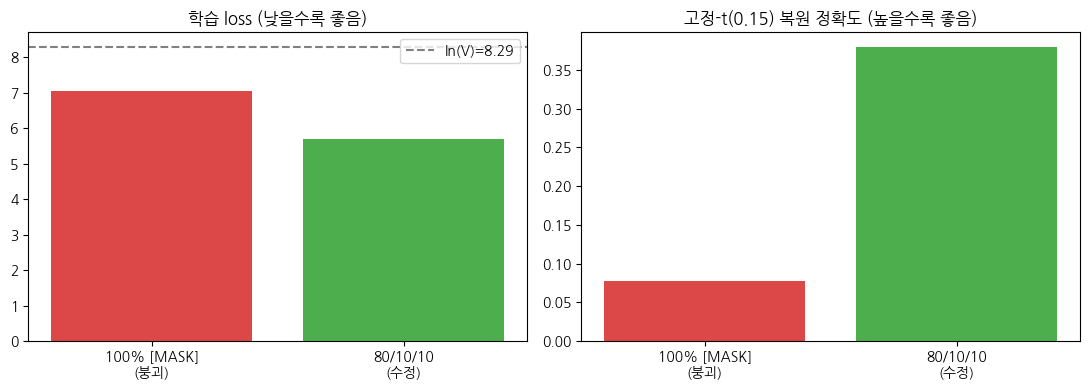
\includegraphics[width=0.86\linewidth]{assets/figures/ch34_masking_ablation.png}
\end{bookfigurelabel}

\textbf{그림 읽기} --- 그림~\ref{fig:ch34-masking-ablation}에서 다음 내용을 확인합니다: 한국어 diffusion 마스킹 방식 비교. 실행된 노트북에서 저장된 최신 plot 출력이므로, 코드에서 계산한 값이 어떤 평가 지점으로 이어지는지 바로 확인할 수 있습니다.



\subsection{정리 --- 무엇을 배웠나}

직접 겪은 순서:

\begin{enumerate}
\def\labelenumi{\arabic{enumi}.}
\tightlist
\item
  \textbf{붕괴 재현}: 영어에서 잘 되던 \emph{100\% \texttt{{[}MASK{]}}} diffusion 을 한국어에 그대로 옮기니, loss 가 유니그램 값에서 평탄 (붕괴).
\item
  \textbf{진단}: 100\% \texttt{{[}MASK{]}} 는 “\texttt{{[}MASK{]}}면 출력, 아니면 베끼기” 라는 \emph{복사 지름길} 을 열어, 모델이 문맥 추론을 안 배움 --- 토큰이 잘게 쪼개지는 한국어에서 특히 치명적.
\item
  \textbf{수정}: 80/10/10(80\% \texttt{{[}MASK{]}} / 10\% 랜덤 / 10\% 원본 유지)으로 그 지름길을 막으니, 모델이 모든 자리에서 문맥을 봐야 해 loss 하락·복원 회복.
\end{enumerate}

\textbf{핵심 교훈}

\begin{itemize}
\tightlist
\item
  \textbf{“한 가지만 바꿨다”의 함정.} “언어만 바꿨다”고 생각했지만, 영어 레시피를 옮기는 과정에서 \emph{80/10/10이라는 숨은 전제} 가 함께 빠져 있었습니다. 내가 \emph{정말 무엇을 바꿨는지} 를 끝까지 의심해야 합니다.
\item
  \textbf{고전이 답일 때가 많습니다.} 80/10/10은 2018년 BERT 논문에 이미 있던 트릭입니다. 새 알고리즘(diffusion)에 옛 지혜가 빠졌던 것뿐입니다.
\item
  같은 데이터·모델·step·loss 인데 \emph{마스킹 방식 하나} 로 붕괴와 정상이 갈렸습니다. 본 장이 80/10/10 을 쓴 이유가 바로 이것입니다.
\end{itemize}